\section*{Обработка результатов:}
\begin{enumerate}
    \item 
    \begin{align*}
        &R = \frac{\lambda}{\delta\lambda} = b \frac{dn}{d\lambda} \\
        &D = \frac{m}{\sqrt{d^2 - m^2 \lambda^2}} \\
        &m \cdot N = R \\
        &N = d \cdot n, \\
    \end{align*}
    где $m$ --- максимумы, $d = 1/n, n = 100$ штр/мм, $d$ --- длинна решетки. 
    
    \item Для каждой длинны волны определим показатель преломления: \\
    \begin{tabu} to 1\textwidth{|c|c|c|c|c|}
    \hline
    \lambda, nm & 404,7 & 491,6 & 546,1 & 578 \\
    \hline
    \delta  & 63\degree32'52" & 65\degree21'52" & 64\degree46'54" & 63\degree56'54" \\
    \hline
    $n$     & 1,7179    & 1,7315    & 1,7272    & 1,7209 \\
    \hline
    \end{tabu}
    
    \item Соответсвие длинн волн и показателя преломления: \\
    \begin{tabu}{|c|c|c|}
        \hline
        \lambda, nm & $n$ & \\
        \hline
        589,3 & 1,67 & d \\
        \hline
        486,1 & 1,72 & f \\
        \hline
        656,3 & 1,7 & c \\
        \hline
    \end{tabu}
    
    \item Найдем среднюю диспрсию и коэффициент диспрсии: \\
    $D = 0,02$ \\
    $\nu = 33,5$
    
    \item Найдем разрешающую способность призмы: \\
    $R = \frac{\lambda}{\delta\lambda} = 1964,33$ \\
    $b_\text{рабочая} = 0,039$ \\
    $R = b \frac{dn}{d\lambda} = 3500$

    \item И наконец, построим график зависимости $n(\lambda)$:
    \begin{figure}[h!]
        \noindent\centering{
            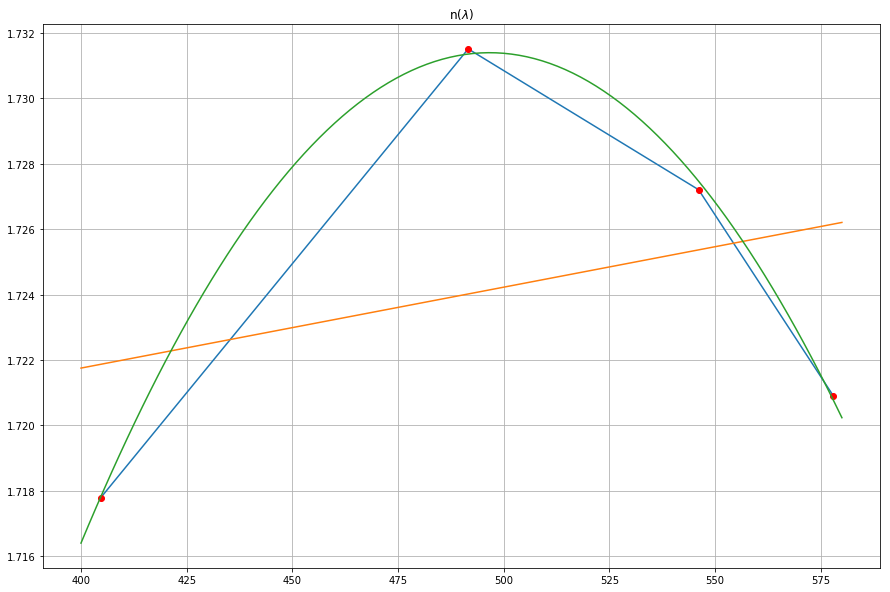
\includegraphics[height = 10cm]{3.png}
        }
    \end{figure} \\
    
\end{enumerate}
